\documentclass[varwidth,border=7mm]{standalone}
\usepackage{tikz}
\usetikzlibrary{decorations.pathreplacing}
\usetikzlibrary{arrows.meta}
\usetikzlibrary{calc}
\tikzset{
  int/.style={
    decoration={brace,mirror,raise=5pt},
    postaction={decorate,draw,blue,-},
  },
  intname/.style = {pos=.5,below=11pt,blue,inner sep=0},
  pt/.style={above left,inner sep=2pt,font=\small},
  yl/.style={inner sep=1pt,fill=white,font=\small,text=orange},
  val/.style={left,inner sep=1pt}
}
\begin{document}
  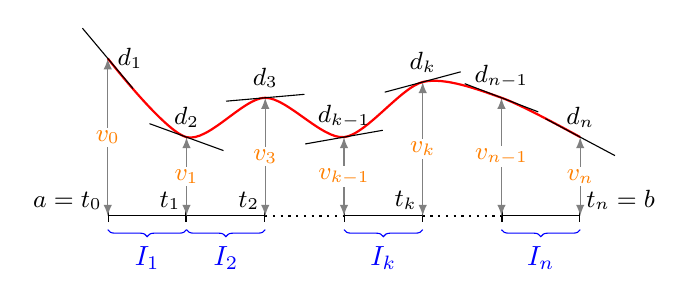
\begin{tikzpicture}
    \draw[int,|-|] (0,0) node[pt]{$a=t_{0}$}-- +(1,0) node[intname]{$I_1$} node[pt]{$t_{1}$};
    \draw[gray,latex-latex] (0,0) -- node[yl]{$v_0$} +(0,2) coordinate(v1);

    \draw[int,-|] (1,0) -- +(1,0) node[intname]{$I_2$} node[pt]{$t_{2}$};
    \draw[gray,latex-latex] (1,0) -- node[yl]{$v_1$} +(0,1) coordinate(v2);

    \draw[dotted,thick] (2,0) -- +(1,0);
    \draw[gray,latex-latex] (2,0) -- node[yl]{$v_3$} +(0,1.5) coordinate(v3);

    \draw[int,|-|] (3,0) -- +(1,0) node[intname](Ik){$I_k$} node[pt]{$t_{k}$};
    \draw[gray,latex-latex] (3,0) -- node[yl]{$v_{k-1}$} +(0,1) coordinate(vk);
    \draw[gray,latex-latex] (4,0) -- node[yl]{$v_k$} +(0,1.7) coordinate(vk1);


    \draw[dotted,thick] (4,0) -- +(1,0);

    \draw[int,|-|] (5,0) -- +(1,0) node[intname]{$I_n$} node[pt,above right]{$t_{n}=b$};
    \draw[gray,latex-latex] (5,0) -- node[yl]{$v_{n-1}$} +(0,1.5) coordinate(vn);

    \draw[gray,latex-latex] (5,0) ++(1,0) -- node[yl]{$v_n$} +(0,1) coordinate(vn1);

    \draw[thick, red, smooth] plot coordinates {(v1) (v2) (v3) (vk) (vk1) (vn) (vn1)};
    \foreach \i/\j/\a/\pos in {1/1/-50/right,2/2/-20/above,3/3/5/above,k/k-1/10/above,k1/k/15/above,n/n-1/-21/above,n1/n/-28/above}
      \draw (v\i) node[font=\small,\pos]{$d_{\j}$} +(\a:-.5) -- +(\a:.5);
  \end{tikzpicture}
\end{document}
